% *******************************************************************************
% * Copyright (c) 2008 by Elexis
% * All rights reserved. This document and the accompanying materials
% * are made available under the terms of the Eclipse Public License v1.0
% * which accompanies this distribution, and is available at
% * http://www.eclipse.org/legal/epl-v10.html
% *
% * Contributors:
% *    G. Weirich
% *
% *  $Id: update14.tex 4895 2009-01-02 07:16:49Z rgw_ch $
% *******************************************************************************

% !Mode:: "TeX:UTF-8" (encoding info for WinEdt)

\documentclass[a4paper]{scrartcl}

\usepackage{german}
\usepackage[utf8]{inputenc}
\usepackage{makeidx}
\usepackage[pdftex]{graphicx}
\DeclareGraphicsExtensions{.pdf,.jpg,.png}

\makeindex


\usepackage{floatflt}
\usepackage[]{hyperref}
\usepackage{color}

\begin{document}
\title{Elexis - Update auf 1.4.0}
\author{G. Weirich}

\maketitle
\tableofcontents

\section{Wann und für wen?}
Das Update auf Version 1.4 wird allen Elexis-Anwendern empfohlen. \textbf{Bitte beachten Sie hierzu die Update-Anleitung auf S. \pageref{update}}. Der beste Zeitpunkt ist dann, wenn Sie einen möglichst grossen Teil Ihrer noch offenen Behandlungen angerechnet haben, oft also der Anfang des Neuen Jahres.

\section{Was ist neu?}
Neben Fehlerbehebungen enthält die Version 1.4 wieder einige Neuerungen:

\subsection{Neuer Look}
Die Icons der ersten Elexis-Versionen waren jeweils bei Bedarf 'irgendwo' zusammengesucht worden, und das sah man dem Programm auch an. Mit Version 1.4 wurde ein einheitliches Design angestrebt (Vgl. Abb. \ref{fig:modern}). Wer allerdings lieber den alten Look hat, kann auch wieder zurückschalten\footnote{Eine austauschbare Oberfläche nennt man neudeutsch auch 'plaf' (pluggable look and feel)}.

\begin{figure}
%\begin{minipage} {0.5\textwidth}
    \center
  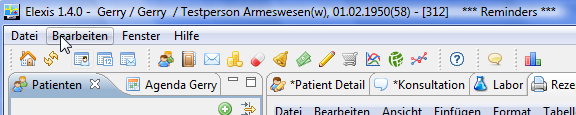
\includegraphics[width=0.7\textwidth]{modern}
  \caption{'Modern' Look}\label{fig:modern}
\end{figure}

%\end{minipage}
%\begin{minipage}{0.5\textwidth}
\begin{figure}
\center
  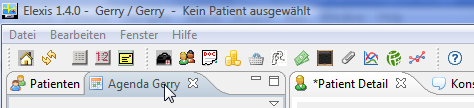
\includegraphics[width=0.7\textwidth]{classic}
  \caption{'Classic' Look}\label{fig:modern}
\end{figure}

\bigskip
Umschalten kann man, indem man Elexis einen Startparameter mit dem gewünschten plaf mitgibt:

\begin{itemize}
\item elexis - -plaf=rsc/plaf/modern  (neues Aussehen)
\item elexis - -plaf=rsc/plaf/classic (klassisches Aussehen)
\end{itemize}

Eine einmal gewählte Oberfläche bleibt gespeichert bis zu einem erneuten expliziten Umschalten. Man braucht den Parameter also nicht jedesmal beim Start zu übergeben.

\subsection{Änderungen am Abrechnungssystem}
\subsubsection{Abrechnungsvorschlag}
\begin{figure}
  % Requires \usepackage{graphicx}
  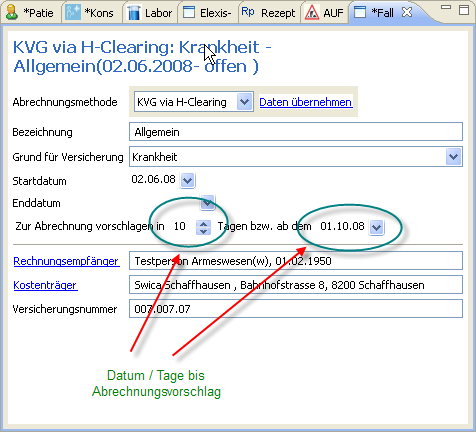
\includegraphics{abrvor1}\\
  \caption{Abrechnungsvorschlag}\label{fig:abrvor1}
\end{figure}

\begin{figure}
  % Requires \usepackage{graphicx}
  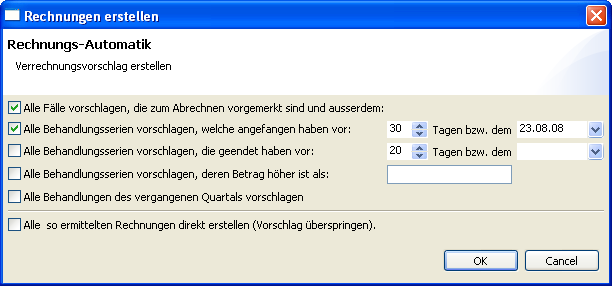
\includegraphics{abrvor2}\\
  \caption{Abrechnungsauswahl}\label{fig:abrvor2}
\end{figure}

Man kann im Fall-Detail (Abb. \ref{fig:abrvor1}) jetzt angeben, dass ein Fall ab einem bestimmten Datum oder nach einer festgelegten Zahl von Tagen zur Abrechnung vorgeschlagen werden soll. Beispielsweise kann man im Notfalldienst einstellen, dass der Fall nach 10 Tagen abgerechnet wird etc. Beim Abrechnen kann man sich dann alle Fälle anzeigen lassen, die entsprechend dieser Vorgaben fällig sind (Abb. \ref{fig:abrvor2}). Wie man hier auch sieht, sind die Datumsfelder so erweitert worden, dass man entweder eine Zahl von Tagen oder ein Stichdatum eingeben kann.

Ausserdem kann man, durch Anklicken des untersten Felds, die Rechnungen direkt ohne weitere Rückfragen und Kontrollmöglichkeiten erstellen lassen.

\subsubsection{\%-Zuschläge und -Abzüge}
Diese wurden früher nicht standardkonform gehandhabt. Dies wurde jetzt korrigiert, so dass beispielsweise Position 35.0020 jetzt korrekt als  Leistung in Höhe der TL der dazugehörigen 'Sparte OP-I' - Leistungen mit  einem Scale-Factor von -0.4 gerechnet wird.

\textbf{Wichtig} Diese Änderung ist der Grund dafür, warum es empfehlenswert ist, den Update auf 1.4 nach erfolgter Abrechnung zu machen: Alle Leistungen, die solche \%-Zuschläge oder -Abzüge enthalten, welche mit Elexis 1.3.x verrechnet wurden, werden nicht korrekt in eine von 1.4.x erstellte Rechnung übernommen. Falls Sie dennoch den Update machen wollen, obwohl noch derartige Abrechnungen offen sind, dann müssen Sie \textit{nach} dem Update auf 1.4 die entsprechenden \%-Positionen aus der Konsultation entfernen und neu verrechnen. Dann wird die Rechnung korrekt erstellt.

\subsubsection{Leistungsdetails (Seite, Pflichtleistung)}
\begin{figure}
  % Requires \usepackage{graphicx}
  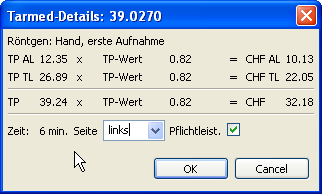
\includegraphics{tarmeddetail1}\\
  \caption{Detail zu Leistung}\label{fig:detail1}
\end{figure}

Man kann jetzt neu zu verrechneten Leistungen Details eingeben (Abb. \ref{fig:detail1}), indem man die betreffende Leistung im Abrechnungsfeld rechts anklickt und 'Details' wählt (Ist nur bei solchen Leistungen anwählbar, wo Details sinnvoll sind). Hier kann man beispielsweise rechts oder links eintragen wo relevant, oder man kann eine Leistung zur Nichtpflichtleistung erklären (Beispielsweise eine von Patienten gewünschte, medizinisch nicht indizierte Ultraschalluntersuchung).

\subsubsection{Adressat in Rechnungdetail-View sichtbar}
In der Rechnungsdetaiö-Ansicht sieht man jetzt auch, an wen die Rechnung adressiert war.

\subsection{Fixmedikation}
(Abb. \ref{fig:fixmedi})
\begin{figure}
  % Requires \usepackage{graphicx}
  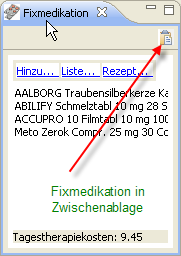
\includegraphics{fixmedi3}\\
  \caption{Fixmedikation}\label{fig:fixmedi}
\end{figure}

\begin{itemize}
\item Zeigt jetzt die Tagestherapiekosten an (Dies geht nur, sofern die Packungsgrösse und die Einnahmefrequenz der Medikamente bekannt sind)
\item Kann die Fixmedikation in die Zwischenablage kopieren, beispielsweise um sie in einen Brief oder den Konsultationstext einzufügen.
\end{itemize}

\subsection{Rezepte}
Mann jetzt auch im Rezept (wie bisher bereits schon bei der Fixmedikation) durch Rechtsklick auf einen Artikel Details zur Verschreibung eingeben wie Einnahmeart und Anweisungen (Abb. \ref{fig:einnahme1}).
\begin{figure}
  % Requires \usepackage{graphicx}
  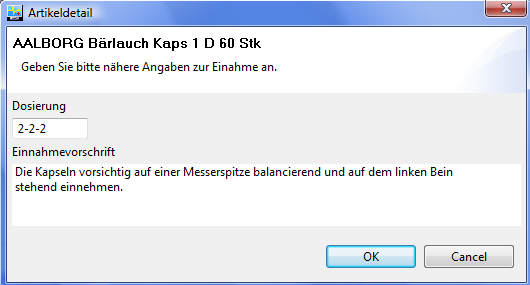
\includegraphics{einnahme1}\\
  \caption{Rezpet: Detailangaben}\label{fig:einnahme1}
\end{figure}

\subsection{Kontaktselektor}
\begin{figure}
  % Requires \usepackage{graphicx}
  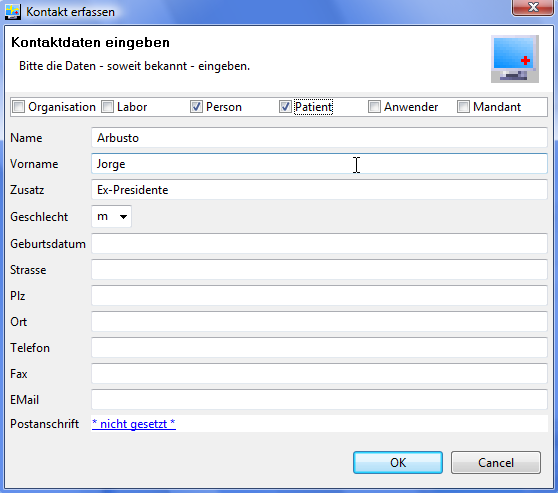
\includegraphics{kontakt}\\
  \caption{Kontakteingabe}\label{fig:kontakt}
\end{figure}

Immer dann wenn ein Kontakt ausgewählt werden soll (z.B. als Adressat von Briefen) kann jetzt auch gleich direkt ein neuer Kontakt inklusive Anschrift erstellt werden. (Abb. \ref{fig:kontakt})

\subsection{Laborimporter}
Die Laborimporter auf HL7-Basis wurden verbessert, so dass jetzt auch Histologie- und Zytologie-Resultate 'vernünftig' formatiert erscheinen sollten.

\subsection{Basis}
Eine Neuerung, die Sie vielleicht nicht auf den ersten Blick bemerken, die aber viel zur Programmstabilität und Detailverbesserungen beiträgt: Elexis basiert jetzt neu auf der aktuellen Eclipse-Version 3.4 (Ganymede).

\subsection{Diverses}
Diverse Details, denen hier kein eigenes Kapital gewidmet werden muss, bzw. die schon früher dokumentiert worden sind.

\section{Upate-Anleitung}
\label{update}
\subsection{Inhaber eines Wartungsvertrags und argoLEAD-Teilnehmer}
Das Update auf 1.4 erfolgt \textit{nicht} automatisch mit dem Update-Programm, sondern muss manuell erfolgen. Wenn Sie einen Wartungsvertrag bei Elexis haben, brauchen Sie nichts zu unternehmen: Das Update gehört zum Leistungsumfang. Wir werden uns unaufgefordert wegen eines Termins bei Ihnen melden, damit wir die Installation vornehmen können. Falls Sie einen Wartungsvertrag bei einem anderen Anbieter haben, fragen Sie bitte dort nach, ob das Update im Preis eingeschlossen ist. Falls Sie Teilnehmer des argoLEAD-Projektes sind und Elexis weiterhin verwenden möchten, werden wir auf Wunsch das Update auf 1.4 per Projektabschluss noch vornehmen (Entweder per Fernzugriff oder bei einem Besuch).

\subsection{Do it yourself}
Machen Sie das Update bitte nur dann selber, wenn Sie sich genug Zeit nehmen können, und wenn Sie sich auch zutrauen, bei einem allfälligen Problem die alte Version wiederherzustellen. Im Zweifelsfall lassen Sie es besser von Ihrem Dienstleister machen.

\medskip

Es ist wichtig, dass keine gemischten Installationen mit 1.3.x und 1.4.x Plugins entstehen. Beachten Sie ausserdem, dass 1.3.x - Plugins oft nicht mehr mit 1.4.x funktionieren werden. Wir empfehlen folgendes Vorgehen:

\begin{enumerate}
\item Falls Sie gekaufte Zusatzplugins von Elexis haben, schreiben Sie eine Mail an support$@$elexis.ch mit einer Auflistung dieser Plugins. Sie erhalten die Updates auf 1.4 kostenlos.  Falls Sie gekaufte Zusatzplugins von anderen Anbietern haben, erkundigen Sie sich bei diesen Anbietern, ob die Plugins mit 1.4 lauffähig sind, bzw. zu welchen Bedingungen ein Update erfolgt.

\item Machen Sie das Update nach Praxisschluss, wenn Sie mindestens eine Stunde Zeit haben. Machen Sie es nur dann selbst, wenn Sie sich ggf. auch zutrauen, das System wieder auf den alten Stand zu bringen, falls etwas nicht gelingt. Das Update muss auf allen Arbeitsstationen separat erfolgen. Gemischter Betrieb von 1.3.x und 1.4.x an derselben Datenbank ist nicht möglich.
\item Machen Sie eine komplette Sicherung der Datenbank und der vorhandenen Elexis-Installationsverzeichnisse. \textbf{Überspringen Sie diesen Schritt nicht, es ist die einzige Möglichkeit, bei einem verunglückten Update wieder zurückzukommen.}
\item laden Sie den Installer von Elexis 1.4 für Ihr Betriebssystem von www.elexis.ch herunter.
\item Benennen Sie das das vorhandene Verzeichnis um. Wenn Elexis in c:$\backslash$Programme$\backslash$elexis installiert ist, nennen Sie es z.B c:$\backslash$Programme$\backslash$elexis-alt. \textbf{Wichtig}: Nicht etwa kopieren, sondern umbenennen. Das Verzeichnis c:$\backslash$Programme$\backslash$elexis darf danach nicht mehr existieren.
\item Starten (Windows) bzw. entpacken (Linux, Mac) Sie den Installer und wählen Sie als Installationsziel den Ort, an dem Elexis vorher installiert war (also im vorigen Beispiel c:$\backslash$Programme$\backslash$elexis). Auf diese Weise wird sichergestellt, dass alle internen und externen Referenzen gültig bleiben und nichts neu konfiguriert werden muss.
\item starten Sie Elexis auf zunächst nur einer der Abeitsstationen und haben Sie ein wenig Geduld: Da die Datenbank reorganisiert wird, kann der erste Start bis 10 Minuten lang dauern, bevor das Elexis-Fenster erscheint.
\item Starten Sie dann Elexis probeweise auf allen Arbeitsstationen. Testen Sie insbesondere auch, ob Sie Rezepte etc. drucken können, damit Sie etwaige Probleme nicht erst am nächsten Arbeitstag bemerken.
\item Wenn alles normal läuft, installieren Sie allfällige Zusatzplugins (wie gesagt in einer für Elexis 1.4 zertifizierten Version).
\end{enumerate}

\subsubsection{Wenn etwas schief gegangen ist}
Wie immer kann man bei Computern nie garantieren, dass alles bei allen so klappt, wie man es sich vorgestellt hat. Daher braucht man eine Möglichkeit, zumindest wieder auf die alte Version zurückzuschalten, damit man weiterarbeiten kann. Da Elexis 1.4 die Datenbank etwas verändert, wird kein 1.3. Client an dieser Datenbank laufen, sondern wird sich beim Start über die zu neue Version beschweren. Sie müssen also so vorgehen:
\begin{enumerate}
\item Beenden Sie Elexis auf allen Stationen
\item machen Sie ein 'Restore' Ihrer vor dem update angefertigten Datenbanksicherung, um wieder die Datenbank der Version 1.3.x zu erhalten.
\item Löschen Sie die elexis-Verzeichnisse auf allen Arbeitsstationen (Oder benennen Sie sie um, z.B. 'elexis-1.4').
\item Benennen Sie die vorher nach 'elexis-alt' umbenannten Verzeichnisse wieder nach 'elexis' um

\end{enumerate}
Danach läuft Elexis wieder auf der Version vor dem Update. Rufen Sie Ihren Supporter an, um den Update zu einem anderen Zeitpunkt zu machen.

\subsection{Beta-Anwender}
Falls Sie schon die Version 1.4 Beta verwendet hatten, müssen Sie trotzdem den Komplettinstaller herunterladen und wie oben beschrieben neu in ein leeres Verzeichnis installieren. Ein einfaches Update von 1.4 Beta auf 1.4 Release wird mit grosser Wahrscheinlichkeit zu verschiedenen Problemen und 'bockenden' Plugins  führen.

\section{Ausblick}
Elexis darf inzwischen als recht ausgereift und professionell nutzbar betrachtet werden. Wir kommen damit jetzt in einer Phase der Neuausrichtung und funktionalen Weiterentwicklung. Es hat sich gezeigt, dass es angesichts der Komplexität der Materie 'elektronische KG' ohne Support nicht geht und dass für einen professionellen Support auch eine professionelle Organisation notwendig ist. Eine solche braucht eine gewisse finanzielle Basis.

Der Elexis-Kern und die für eine sofort einsetzbare einfache elKG nötigen Plugins werden immer OpenSource und frei erhältlich bleiben, aber Wartungsverträge sollen gegenüber der Gratisversion an Attraktivität gewinnen, so dass der mit der Anwenderzahl steigende Supportbedarf finanziert werden kann, damit die Kapazität des immer noch sehr kleinen Elexis-Kernteams auf Produktweiterentwicklungen statt auf Supportleistungen konzentriert werden kann. Es soll sich für den Anwender also doppelt lohnen, einen regelmässigen Jahresbeitrag zu leisten: Einmal darin, dass er definierte Mehrleistungen gegenüber dem Gratis-Nutzer bekommt, und einmal darin, dass er hilft, die Weiterentwicklung seines Praxisprogramms zu fördern, und von Neuerungen auch rascher profitiert. Auch soll es möglich sein, dass Elexis-Anwender Anteile/Aktien der Trägerorganisation erwirbt und auch hier Vorteile gegenüber dem Gratis-Nutzer haben kann.

\medskip

In der Pipeline ist inzwischen Elexis 2.0 mit einer ganzen Reihe von z.T. grundlegenden Neuerungen. Wenn Sie auf dem Laufenden gehalten werden möchten, haben Sie folgende Möglichkeiten: Entweder Sie schauen ab und zu auf der Website (http://www.elexis.ch) oder im elexis-forum (http://www.elexis-forum.ch\footnote{Beim Forum können Sie auch einen RSS-Feed abonnieren, damit Sie automatisch über neue Nachrichten informiert werden}) vorbei, oder Sie lassen Sich auf die Mailing-Liste setzen, dann werden Sie automatisch über relevante News informiert (Mail an support$@$elexis.ch genügt zum An- oder Abmelden).

\medskip

Ihre Fragen, Anregungen und Bemerkungen an support$@$elexis.ch sind willkommen und werden wie immer raschestmöglich beantwortet.

\end{document}
